\documentclass{beamer}
\mode <presentation>
{
    \usetheme{Antibes}
    \usecolortheme{crane}
    \setbeamercovered{transparent}
}

\usepackage[english]{babel}
\usepackage{times}
\usepackage{amsmath}
% math extension - one probably wants to use symbols like '[' (written as '$[$')
\usepackage{ucs}
%\usepackage[utf8]{inputenc}
\usepackage[utf8x]{inputenc}
\usepackage[normalem]{ulem}

%\setbeamercolor{background canvas}{bg=
\includegraphics[width=\textwidth]{./pics/wolf.png}}

\title{Assets management with~FusionInventory~and~GLPI}
\author{\href{http://www.FusionInventory.org}{FusionInventory.org}}
\subject{Assets management with FusionInventory and GLPI}
\keywords{Assets management, Inventory, FusionInventory, GLPI}

\date{
\includegraphics[height=0.3cm]{./pics/cc-by-sa.png} ~ 6th February, 2011}
\titlegraphic{}
%subtitle{
\includegraphics[width=1.2cm]{./pics/fusioninventory-logo.png}}
\institute{
\includegraphics[height=4.2cm]{./pics/fusioninventory-logo.pdf}}
\author{ FusionInventory project }
\logo{
\includegraphics[height=0.7cm]{./pics/fusioninventory-logo.pdf}}

\AtBeginSection[] % Do nothing for \section*
{
    \begin{frame}<beamer>
        \frametitle{Outline}
        \tableofcontents[currentsection]
    \end{frame}
}

%%%%%%%%%%%%%%%%%%%%%%%%%%%%%%%%%%%%%%%%%%%%%%%
%%%%%%%%%%%%%%%%%%%%%%%%%%%%%%%%%%%%%%%%%%%%%%%
\begin{document}

\frame[plain]{\titlepage}


\section{Overview}

\begin{frame}
    \frametitle{Global overview}

    \begin{itemize}
        \item here a schema
    \end{itemize}
\end{frame}

\section{The code}

\subsection{Agent side}
%
\begin{frame}
    \frametitle{Agent history}

    \begin{center}
    
\includegraphics[height=3.5cm]{./pics/agent-smith.jpg}
    \end{center}


    \begin{itemize}
        \item a fork of OCS Inventory UNIX agent by its author
        \item started 5 years ago
        \item GPLv2
    \end{itemize}
\end{frame}

\begin{frame}
    \begin{center}
    
\includegraphics[height=4.0cm]{pics/Perl_Foundation.pdf}
    
\includegraphics[height=4.0cm]{pics/yoda.jpg}
    \end{center}
    \frametitle{use Perl Luke!}

    We choose to use Perl on the agent side.
    \begin{itemize}
        \item portable
        \item reliable
        \item versatile
        \item stable API, Oh my!
    \end{itemize}
\end{frame}

\begin{frame}
    \frametitle{Agent push}


    
\includegraphics[height=4.0cm]{pics/kung-fu-panda.jpg}


    AKA: The agent hits first!

\end{frame}

\begin{frame}
    \frametitle{Server pull}

    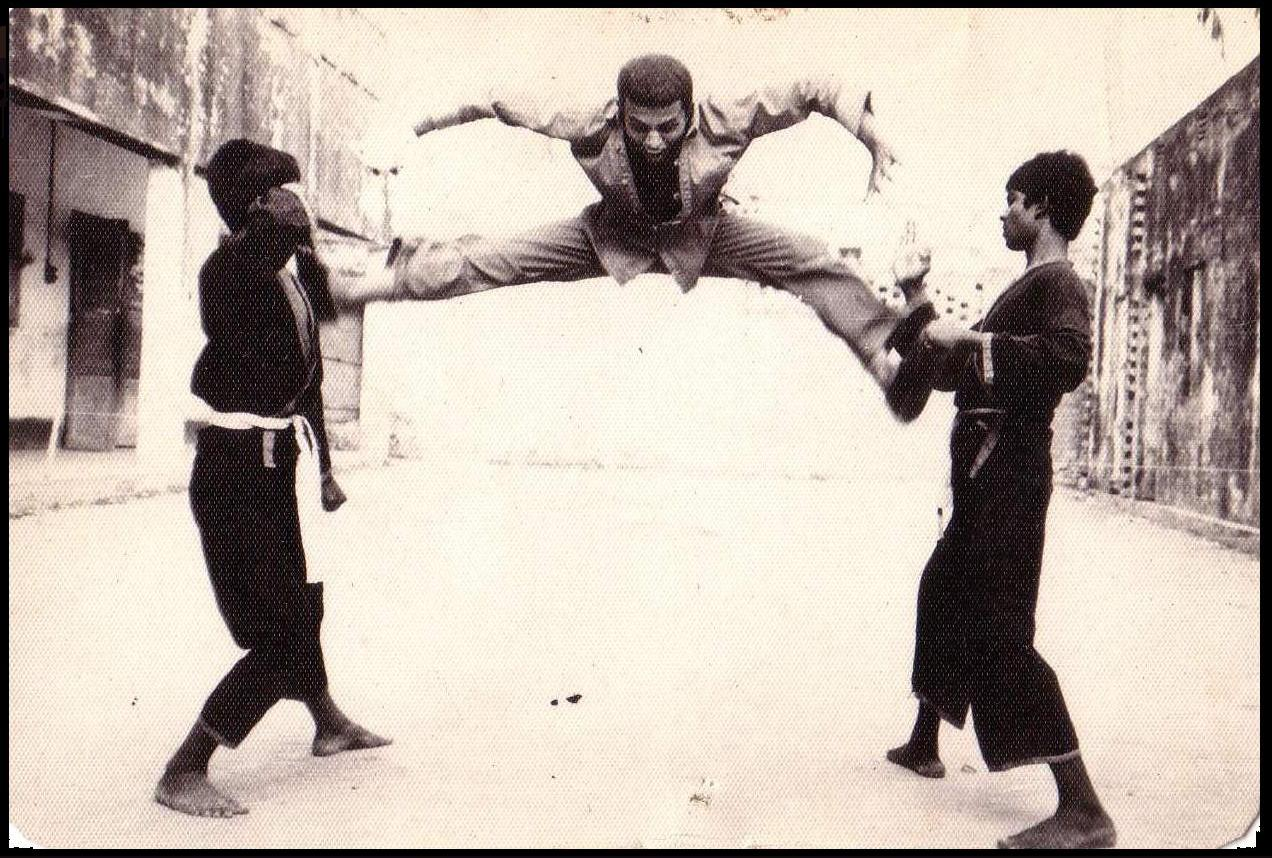
\includegraphics[height=5.0cm]{pics/double-kick.jpg}


    The server hits the agents first! \small{and the agents hit back!}

\end{frame}

\begin{frame}
    \frametitle{Task}
    %
    Not only for local machine inventory. The agent supports different "tasks".

    \pause
    \begin{itemize}

        \item Network discovery
        \item Remote inventory
        \item Software deployment
        \item Wake On Lan
        \item ...
    \end{itemize}
\end{frame}

\begin{frame}
    \frametitle{The inventories}

    \begin{description}
        \item[BIOS] serial numbers, UUID, etc local
        \item[Memory] memory slot, size, etc
        \item[CPU] frequency, name, manufacturer, etc
        \item[Software] apt-get, yum, Windows software, BSD pkg, etc
        \item[Harddrive] serial number, manufacturer, etc
        \item[Partition] etc
        \item[Virtual Machine] libvirt, xen, etc
        \item[USB devices] phone, USB key, etc
        \item[etc] \href{http://search.cpan.org/dist/FusionInventory-Agent/lib/FusionInventory/Agent/XML/Query/Inventory.pm}{see the list on Internet.}
    \end{description}

    It's easy to add new information. Just ask us or submit patches!

\end{frame}

\begin{frame}
    \frametitle{Network discovery}

    \begin{itemize}
        \item TODO
    \end{itemize}
\end{frame}

\begin{frame}
    \frametitle{Remote inventory}

    \begin{block}{Network devices}
        \begin{itemize}
            \item serial number, firmware, ...
            \item ports mapping
        \end{itemize}
    \end{block}

    \begin{block}{Network printers}
        \begin{itemize}
            \item serial number, firmware, ...
            \item cartridge ink level
        \end{itemize}
    \end{block}
\end{frame}

\begin{frame}
    \frametitle{Wake on LAN}

    \begin{itemize}
        \item TODO
    \end{itemize}
\end{frame}

\begin{frame}
    \frametitle{Software deployment}

    \begin{itemize}
        \item TODO
    \end{itemize}
\end{frame}

\begin{frame}
    \frametitle{supported OS (1/2)}

    
\includegraphics[height=4.5cm]{pics/forrest.jpg}
    Runs everywhere!

    \pause

    \begin{block}{FusionInventory Portage for dummies}
        \begin{itemize}
            \item extend the Inventory modules to collect information
            \item and, hum, well, that's all. We're done :D
        \end{itemize}
    \end{block}
\end{frame}

\begin{frame}
    \frametitle{supported OS (2/2)}
    Supported Operating Systems:

    \begin{itemize}
        \item<2-> Linux
        \item<3-> BSD
        \item<4-> AIX
        \item<5-> HP-UX
        \item<6-> Solaris
        \item<7-> Windows, all from 2000 to Seven 64bit
    \end{itemize}


    \uncover<8->{\href{http://forge.fusioninventory.org/projects/fusioninventory-agent/wiki/Agent\_supportedplateforms}{A complete list is avallable on the website}}


\includegraphics[height=0.5cm]{pics/logos/aix.png}

\includegraphics[height=0.5cm]{pics/logos/fedora.png}

\includegraphics[height=0.5cm]{pics/logos/hp-ux.png}

\includegraphics[height=0.5cm]{pics/logos/netbsd.png}

\includegraphics[height=0.5cm]{pics/logos/openbsd.png}

\includegraphics[height=0.5cm]{pics/logos/solaris.jpg}

\includegraphics[height=0.5cm]{pics/logos/centos.jpg}

\includegraphics[height=0.5cm]{pics/logos/linux.png}

\includegraphics[height=0.5cm]{pics/logos/osx.png}

\includegraphics[height=0.5cm]{pics/logos/ubuntu.png}

\includegraphics[height=0.5cm]{pics/logos/debian.png}

\includegraphics[height=0.5cm]{pics/logos/freebsd.png}

\includegraphics[height=0.5cm]{pics/logos/redhat.png}

\includegraphics[height=0.5cm]{pics/logos/windows.jpg}

\includegraphics[height=0.5cm]{pics/logos/dragonflybsd.png}



\end{frame}


\begin{frame}
    \frametitle{Server?}

    \pause

    \begin{block}{The agent supports 3 different servers}
        \begin{description}
            \item FusionInventory for GLPI 0.78
            \item Uranos
            \item OCS Inventory NG
        \end{description}
    \end{block}
\end{frame}



\begin{frame}
    \frametitle{What else?}

    \begin{center}
    
\includegraphics[height=4.0cm]{pics/whatelse.jpg}
    \end{center}

    \pause

    \begin{block}{3.0 branch in active development}
        \begin{itemize}
            \item code clean up\\
            {\small larger test-suite, modern perl}
            \item architecture changes\\
            {\small event-driven programming, various executable}
            \item smaller memory footprint
        \end{itemize}
    \end{block}
\end{frame}




\subsection{Server side}
%
%\logo{
\includegraphics[height=1cm]{./pics/fusioninventory-logo.png}}
%
\subsection{History}
%-------------------------------------------------------------------

\subsection{Internal}
%-------------------------------------------------------------------
\begin{frame}
\frametitle{GLPI plugin}
%
\begin{itemize}
\item FusionInventory for GLPI is ... a plugin for ... GLPI. Wait! What? 
%
\end{itemize}
\end{frame}

%-------------------------------------------------------------------
\begin{frame}
\frametitle{GLPI plugin}
%
\begin{itemize}
\item PHP/MySQL
%
\end{itemize}
\end{frame}

\subsection{Data exchange}
%-------------------------------------------------------------------
\begin{frame}
\frametitle{the protocol}
%
\begin{itemize}
\item HTTPS everywhere! 
%
\end{itemize}
\end{frame}





\subsection{Use cases}
\begin{frame}
    \frametitle{The inventories}

    \begin{description}
        \item[BIOS], serial numbers, UUID, etc local
        \item[Memory], memory slot, size, etc
        \item[CPU], frequency, name, manufacturer, etc
        \item[Software], apt-get, yum, Windows software, BSD pkg, etc
        \item[Harddrive], serial number, manufacturer, etc
        \item[Partition], etc
        \item[Virtual Machine], libvirt, xen, etc
        \item[USB devices], phone, USB key, etc
        \item[etc], \href{http://search.cpan.org/dist/FusionInventory-Agent/lib/FusionInventory/Agent/XML/Query/Inventory.pm}{see the list on Internet.}
    \end{description}

    It's easy to add new information. Just ask us or submit patches!

\end{frame}

\begin{frame}
    \frametitle{Identify devices on the network}

    \begin{itemize}
        \item TODO
    \end{itemize}
\end{frame}

\begin{frame}
    \frametitle{Switch inventory}

    \begin{itemize}
        \item TODO
    \end{itemize}
\end{frame}

\begin{frame}
    \frametitle{printer too!}

    \begin{itemize}
        \item TODO
    \end{itemize}
\end{frame}

\begin{frame}
    \frametitle{Wake on LAN}

    \begin{itemize}
        \item TODO
    \end{itemize}
\end{frame}

\begin{frame}
    \frametitle{Software deployment}

    \begin{itemize}
        \item TODO
    \end{itemize}
\end{frame}

\begin{frame}
    \frametitle{Task Scheduling}

    \begin{itemize}
        \item TODO
    \end{itemize}
\end{frame}

\begin{frame}
    \frametitle{libFusionInventory}
    
    \begin{itemize}
        \item TODO
    \end{itemize}
\end{frame}


\section{The project}

\subsection{History}
\begin{frame}
    \frametitle{A long long time ago}

    Tracker was a GLPI extension with a Perl agent.

    It goal was simple: just “SNMP” inventory
    
\includegraphics[height=2.5cm]{./pics/frog1.pdf}
\end{frame}

\begin{frame}
    \frametitle{A long long time ago again}
    
    OCS Inventory Agent for UNIX was an inventory agent without SNMP support.

    
\includegraphics[height=2.5cm]{./pics/frog2.pdf}
\end{frame}

\begin{frame}
    \frametitle{And they kissed}
    
    And they did some kind of fusion...
    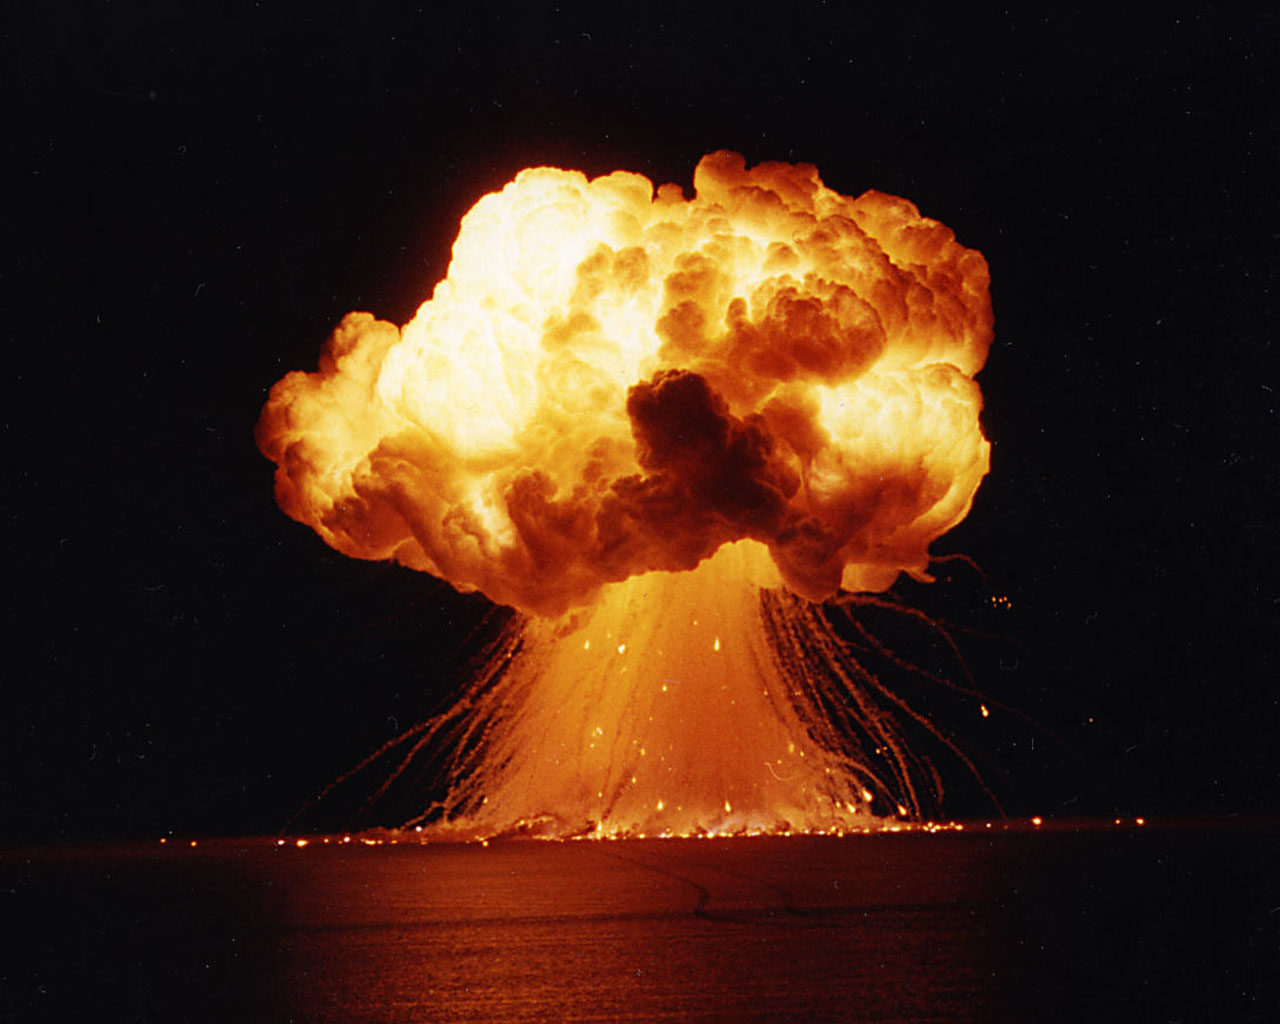
\includegraphics[height=6.5cm]{./pics/explode.jpg}
\end{frame}


\subsection{Community}

\begin{frame}
    \frametitle{The project workflow}
    %%-------------------------------------------------------------------
    %%\logo{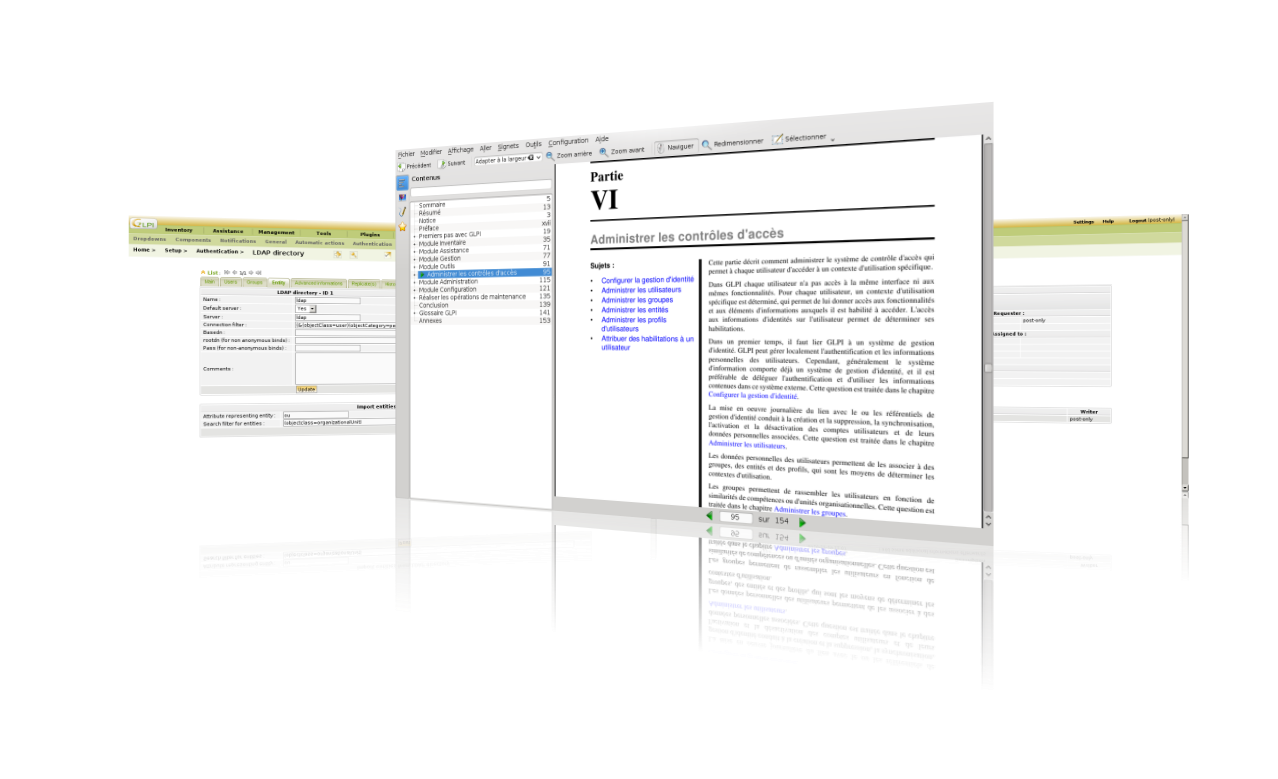
\includegraphics[height=3.5cm]{./pics/glpi-doc.png}}
    FusionInventory is a community driven project.

    \begin{itemize}
        \item active mailing lists
        \item IRC: \#FusionInventory on FreeNode
        \item public Forge, Git repositories, etc
    \end{itemize}
\end{frame}

\begin{frame}
    \frametitle{Who}

    \sout{\bf{We are Legion!}}
    \begin{center}
    
\includegraphics[height=3.5cm]{./pics/sparta.jpg}
    \end{center}

    About 10 people involved in the project and an active community of contributor.

    \pause
    \bf{We are looking for people to JOIN US!}
\end{frame}

\begin{frame}
    \frametitle{Our roadmap}

    What we are about to release in the coming...
    \begin{itemize}
        \item weeks
        \begin{description}
            \item[FusionInventory for GLPI 0.78] bêta planned for XXXX
        \end{description}
        \item months
        \begin{description}
            \item[ESX inventory] release to be synchronized with GLPI 0.81
        \end{description}
        \item no planing deadline yet
    \end{itemize}
\end{frame}

\section{Conclusion}

\begin{frame}
    \frametitle{Question?}
    
    \begin{itemize}
        \item TODO
    \end{itemize}
\end{frame}

%\setbeamertemplate{headline}{
\includegraphics[width=\paperwidth, height=2cm, clip=true]{./pics/header.png}}
%\begin{frame}[plain]
\begin{frame}[shrink=20]{Outline}

    \tableofcontents
\end{frame}
\end{document}
